\documentclass[tikz,border=3mm]{standalone}
\usetikzlibrary{calc, arrows.meta}
\usepgfmodule{nonlineartransformations}

% Define the transformation to be employed
\makeatletter
\def\transformA{%
  \pgfmathsetmacro{\myX}{\pgf@x + 20*sin(-\pgf@y + .7*\pgf@x)}
  \pgfmathsetmacro{\myY}{\pgf@y + 20*cos(% .8\pgf@y +
    \pgf@x)}
  \setlength{\pgf@x}{\myX pt}
  \setlength{\pgf@y}{\myY pt}
}

% \def\transformB{%
  % \pgfmathsetmacro{\myRsq}{1/(sin(\pgf@x)*sin(\pgf@y) + 2)}
  % \pgfmathsetmacro{\myRsq}{1/(.001*\pgf@x*\pgf@x + .001*\pgf@y*\pgf@y + 1)}
  % \pgfmathsetmacro{\myX}{\pgf@x*e^(-\myRsq)}
  % \pgfmathsetmacro{\myY}{\pgf@y*e^(-\myRsq)}
  % \setlength{\pgf@x}{\myX pt}
  % \setlength{\pgf@y}{\myY pt}
% }

\makeatother

\begin{document}
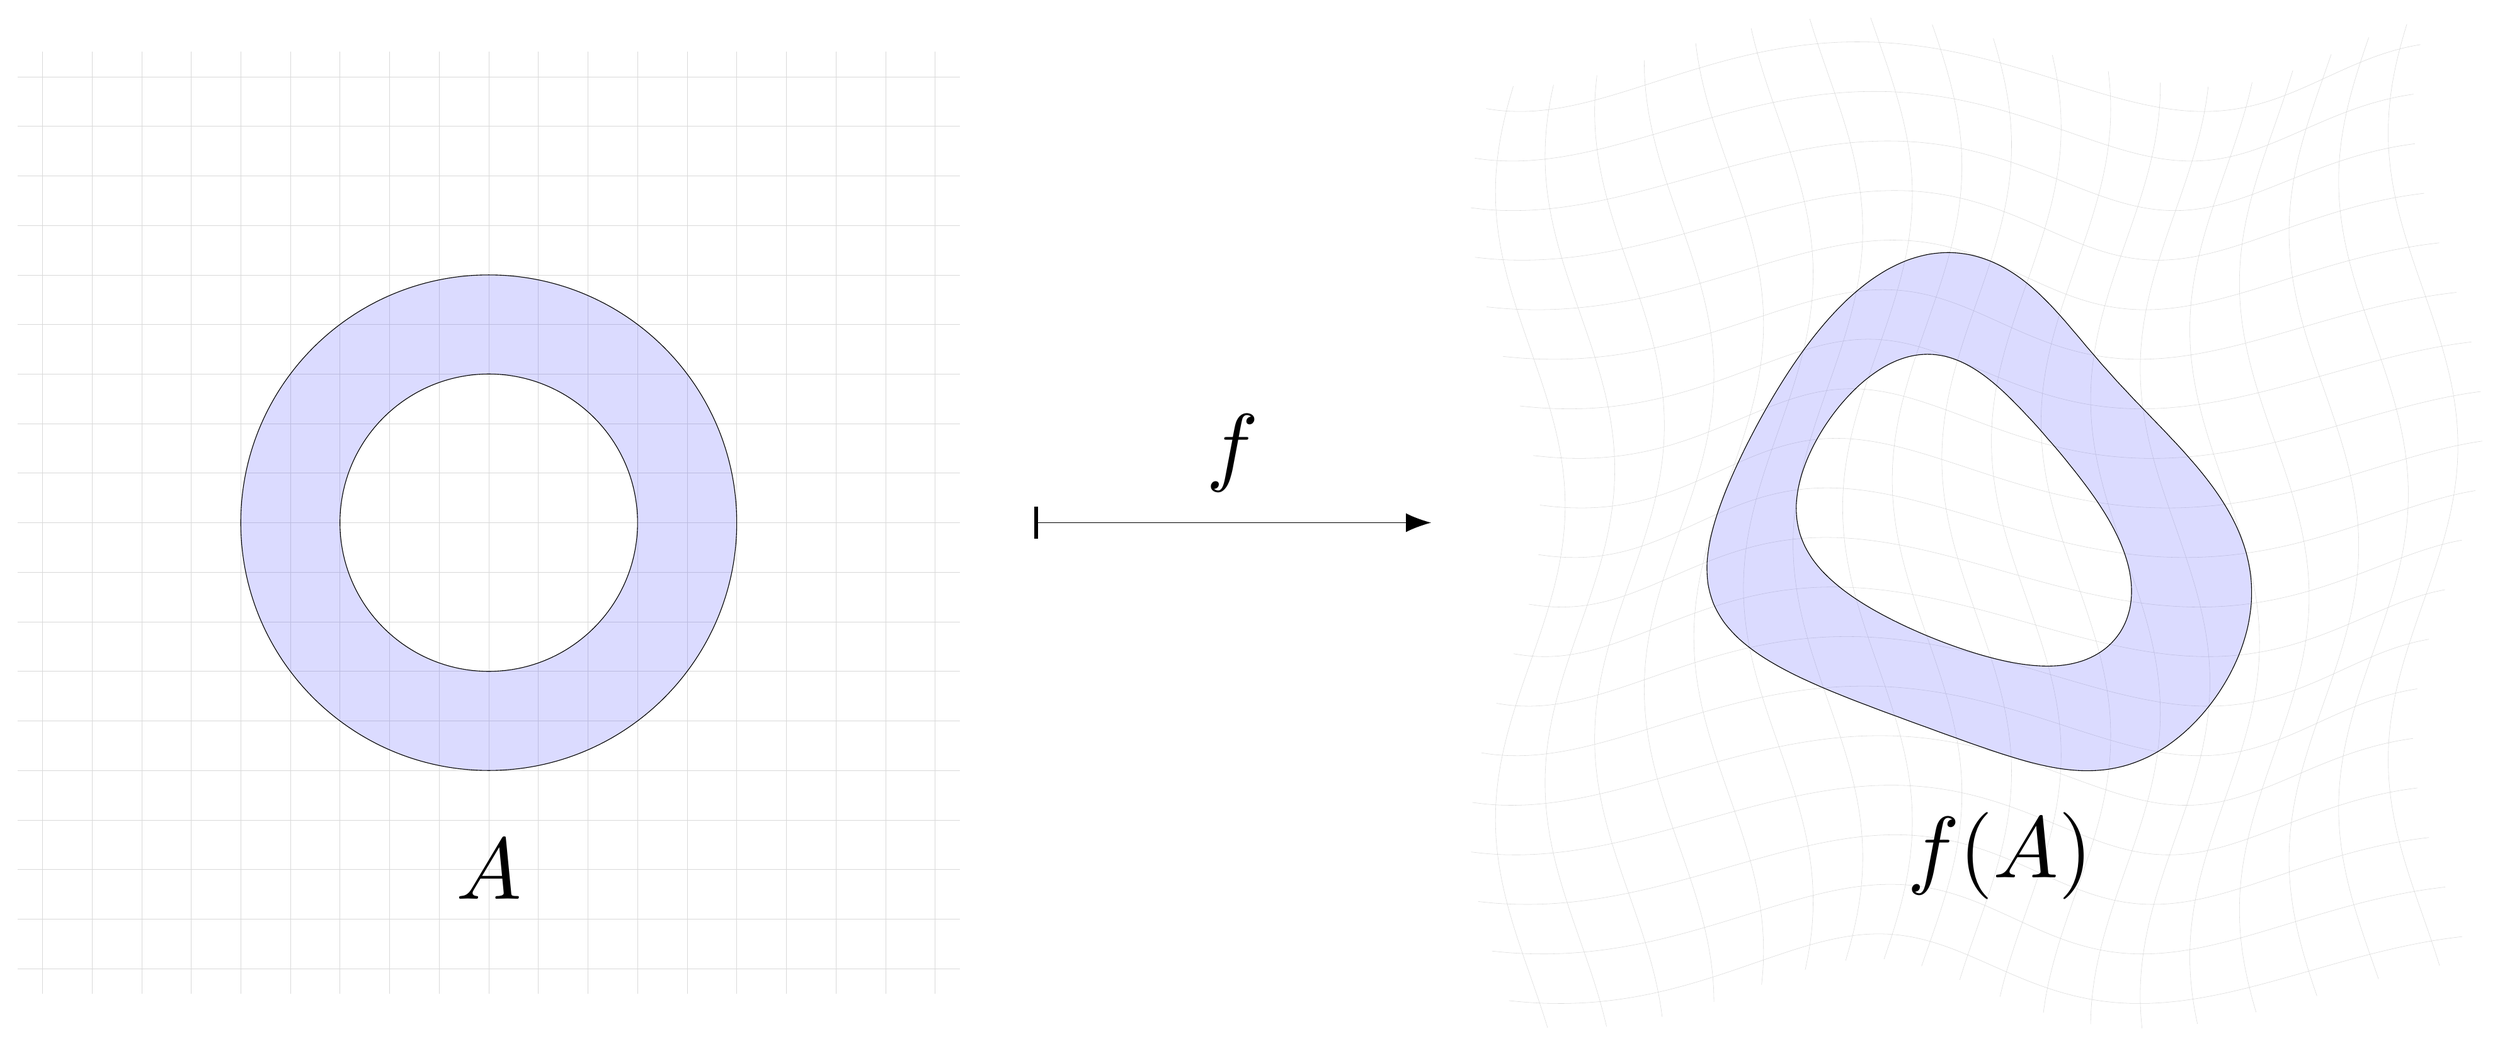
\begin{tikzpicture}[every node/.style={scale=5}]

  % Define xmin xmax ymin ymax
  \pgfmathsetmacro{\xmin}{-10}
  \pgfmathsetmacro{\xmax}{10}

  \pgfmathsetmacro{\ymin}{-10}
  \pgfmathsetmacro{\ymax}{10}

  \def\drawblob{
    \filldraw[draw=black, draw opacity=1, fill=blue!70!white, fill
    opacity=.2, even odd rule] (0,0) circle[radius=2.5cm]
    circle[radius=1.5cm];
  }

  \def\mydraw{
    \draw[help lines, color=gray!30] ($(\xmin, \ymin) + (.5,
    .5)$) grid ($(\xmax, \ymax) + (-.5, -.5)$);
    \begin{scope}[scale=2]% [xshift=-7cm, yshift=10cm, scale=2]
      \drawblob
    \end{scope}
  }

  \begin{scope}[xshift=-15cm]
    \mydraw
    \node () at (0,-7) {$A$};
  \end{scope}
  \draw[{Bar[scale=4, line width=2]}-{Latex[scale=3]}] (-4, 0) -- (4,0) node[midway, above] {$f$};
  \begin{scope}[xshift=15cm]
    \pgftransformnonlinear{\transformA}
    \mydraw
    \node () at (0,-7) {$f(A)$};
  \end{scope}

  % \begin{scope}[xshift=15cm, yshift=-15cm]
  %   \pgftransformnonlinear{\transformB}
  %   \mydraw
  % \end{scope}
% Here back to normal

\end{tikzpicture}


\end{document}
